% !TeX program = lualatex
% ================================================================
% Polish Parallel Text Version of IndicesQuickQuestions
%
% Generated by the server using the following settings:
%
%   language            Polish (pol)
%   text direction      left to right
%   font                Noto Serif
%   fallback font       Noto Serif
%   built from          latex/quickQuestions/indicesQuickQuestions.tex
%   vocabulary key      latex/quickQuestions/indicesQuickQuestions/L2/pol/indicesQuickQuestions_polishKey.tex
%   tier 3 vocabulary   green   RGB 0 128 0
%   English text        black   RGB 0 0 0
%   Polish text         purple  RGB 112 48 160
%   layout macros       version 3
%
% Please don't edit any information in this comment block - the server
% compares it against the current settings and rebuilds this file when
% they differ, so changes here would be overwritten. However, feel free
% to make updates to the LaTeX below if you want to edit it.
% ================================================================

\documentclass[aspectratio=169]{beamer}
% ================================================================
% Copied from the English sheet this was translated from, so that
% anything it sets up for itself still works here
% ================================================================
\usepackage{amsmath}
\usepackage{amssymb}
\usepackage{tikz}
\usetikzlibrary{positioning}

% ================================================================
% Quick Questions deck: index rules.
%
% Each topic opens with five true/false statements and then runs ten
% quick questions that get gradually harder. Every question gets two
% slides: the question on its own for the mini whiteboards, then the
% same question again with the solution underneath in red.
%
% The three green topics work on the index laws themselves, first with
% positive indices, then with negative ones, then applied to algebraic
% expressions. The four amber topics move on to roots: estimating them,
% then indices of the form 1/a and a/b, and finally negative
% fractional indices.
%
% Where the working can be drawn it is: a halving ladder for the
% negative indices, number lines for the estimating, area and volume
% pictures for the square and cube roots, and flow charts for the
% fractional indices, which show the root, the power and the
% reciprocal as separate steps done in order.
% ================================================================

\setbeamertemplate{navigation symbols}{}

% A link in the bottom left of every slide back to the contents, so a
% deck this long can be jumped around in during a lesson.
\setbeamertemplate{footline}{%
  \hbox to\paperwidth{%
    \hspace{1em}%
    \hyperlink{contents}{%
      \color{gray}\scriptsize$\leftarrow$~Back to contents}%
    \hfil}%
  \vskip4pt%
}

% Topic divider.
\newcommand{\qtopic}[1]{%
  \section{#1}%
  \begin{frame}
    \vfill
    \begin{center}
      {\usebeamercolor[fg]{structure}\Huge\bfseries #1}
    \end{center}
    \vfill
  \end{frame}%
}

% \qq[<question size>][<solution size>]{<question>}{<solution>}
% The two optional sizes drop the type for the wordier questions and
% the longer solutions, so nothing runs off the slide.
\NewDocumentCommand{\qq}{O{\Huge}O{\LARGE}+m+m}{%
  \begin{frame}
    \vfill
    \begin{center}
      \begin{minipage}{0.92\textwidth}
        \centering #1 #3
      \end{minipage}
    \end{center}
    \vfill
  \end{frame}%
  \begin{frame}
    \vfill
    \begin{center}
      \begin{minipage}{0.92\textwidth}
        \centering #1 #3
        \par\vspace{0.9em}
        {\color{red}#2 #4}
      \end{minipage}
    \end{center}
    \vfill
  \end{frame}%
}

% \tf[<statement size>][<answer size>]{<statement>}{<answer>}
% As \qq, but with a standing "True or false?" heading above the
% statement. The statements hunt for the usual misconceptions, so the
% answer always says why, not just which.
\NewDocumentCommand{\tf}{O{\LARGE}O{\Large}+m+m}{%
  \begin{frame}
    \vfill
    \begin{center}
      \begin{minipage}{0.92\textwidth}
        \centering
        {\usebeamercolor[fg]{structure}\Large\bfseries True or false?}
        \par\vspace{1em}
        #1 #3
      \end{minipage}
    \end{center}
    \vfill
  \end{frame}%
  \begin{frame}
    \vfill
    \begin{center}
      \begin{minipage}{0.92\textwidth}
        \centering
        {\usebeamercolor[fg]{structure}\Large\bfseries True or false?}
        \par\vspace{1em}
        #1 #3
        \par\vspace{0.9em}
        {\color{red}#2 #4}
      \end{minipage}
    \end{center}
    \vfill
  \end{frame}%
}

% Chained working, one equation per row, so that a long run of index
% laws does not have to be squeezed onto a single line.
\newcommand{\work}[1]{%
  \begin{tabular}{@{}r@{\;=\;}l@{}}#1\end{tabular}%
}

% \flow{<start>}{<first step>}{<middle>}{<second step>}{<end>}
% A flow chart of three boxes joined by two labelled arrows. Used for
% the fractional indices, where the point is that the root and the
% power are separate steps, done one after the other.
\newcommand{\flow}[5]{%
  \begin{tikzpicture}[
      fbox/.style={draw=red!60!black, rounded corners=2pt, fill=red!8,
                   inner sep=5pt, text=red, font=\large},
      farr/.style={->, red, thick, shorten >=1pt, shorten <=1pt}]
    \node[fbox] (a) {$#1$};
    \node[fbox, right=2.4cm of a] (b) {$#3$};
    \node[fbox, right=2.4cm of b] (c) {$#5$};
    \draw[farr] (a) -- node[above,text=red,font=\small]{#2} (b);
    \draw[farr] (b) -- node[above,text=red,font=\small]{#4} (c);
  \end{tikzpicture}%
}

% \flowfour{<start>}{<step>}{<second>}{<step>}{<third>}{<step>}{<end>}
% The same chart with a third arrow, for the negative fractional
% indices, where taking the reciprocal is a step of its own.
\newcommand{\flowfour}[7]{%
  \begin{tikzpicture}[
      fbox/.style={draw=red!60!black, rounded corners=2pt, fill=red!8,
                   inner sep=4pt, text=red, font=\large},
      farr/.style={->, red, thick, shorten >=1pt, shorten <=1pt}]
    \node[fbox] (a) {$#1$};
    \node[fbox, right=2.0cm of a] (b) {$#3$};
    \node[fbox, right=2.0cm of b] (c) {$#5$};
    \node[fbox, right=2.0cm of c] (d) {$#7$};
    \draw[farr] (a) -- node[above,text=red,font=\small]{#2} (b);
    \draw[farr] (b) -- node[above,text=red,font=\small]{#4} (c);
    \draw[farr] (c) -- node[above,text=red,font=\small]{#6} (d);
  \end{tikzpicture}%
}

% The powers of 2 running down from 2^3 to 2^{-3}, halving at every
% step. The negative indices are not a new rule: they are the same
% pattern carried on past 2^0=1.
\newcommand{\halvingladder}{%
  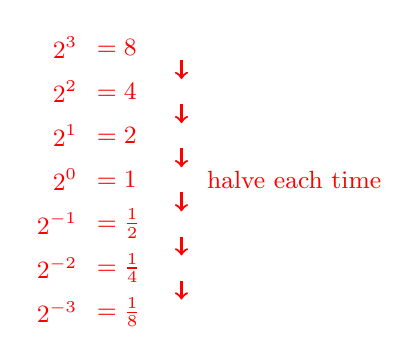
\begin{tikzpicture}[x=1cm,y=1cm,color=red,font=\small]
    \node[anchor=east] at (0,0)    {$2^{3}$};  \node[anchor=west] at (0,0)    {$=8$};
    \node[anchor=east] at (0,-0.56) {$2^{2}$};  \node[anchor=west] at (0,-0.56) {$=4$};
    \node[anchor=east] at (0,-1.12) {$2^{1}$};  \node[anchor=west] at (0,-1.12) {$=2$};
    \node[anchor=east] at (0,-1.68) {$2^{0}$};  \node[anchor=west] at (0,-1.68) {$=1$};
    \node[anchor=east] at (0,-2.24) {$2^{-1}$}; \node[anchor=west] at (0,-2.24) {$=\tfrac{1}{2}$};
    \node[anchor=east] at (0,-2.80) {$2^{-2}$}; \node[anchor=west] at (0,-2.80) {$=\tfrac{1}{4}$};
    \node[anchor=east] at (0,-3.36) {$2^{-3}$}; \node[anchor=west] at (0,-3.36) {$=\tfrac{1}{8}$};
    \foreach \i in {0,...,5}{%
      \draw[->,red,thick] (1.2,{-0.56*\i-0.16}) -- (1.2,{-0.56*\i-0.40});}
    \node[anchor=west,font=\small] at (1.4,-1.68) {halve each time};
  \end{tikzpicture}%
}

% \rootline{<left label>}{<right label>}{<root being estimated>}{<how far along, 0 to 1>}
% A number line running between the two whole numbers either side of a
% root, with the root marked in its true position between them.
\newcommand{\rootline}[4]{%
  \begin{tikzpicture}[x=1cm,y=1cm]
    \draw[red!55!black,thick] (0,0) -- (9,0);
    \draw[red!55!black,thick] (0,-0.16) -- (0,0.16);
    \draw[red!55!black,thick] (9,-0.16) -- (9,0.16);
    \node[red!55!black,below=6pt,font=\small] at (0,0) {$#1$};
    \node[red!55!black,below=6pt,font=\small] at (9,0) {$#2$};
    \fill[red] ({9*#4},0) circle (2.6pt);
    \node[red,above=5pt,font=\small] at ({9*#4},0) {$#3$};
  \end{tikzpicture}%
}

% \areasquare{<side>}{<area>} — a square labelled with its area and the
% side length that gives it. The square root of a number is the side of
% the square with that area, which is what the picture is there to say.
\newcommand{\areasquare}[2]{%
  \begin{tikzpicture}[x=1cm,y=1cm]
    \draw[red!60!black,thick,fill=red!8] (0,0) rectangle (2.4,2.4);
    \node[red,font=\small] at (1.2,1.2) {area $#2$};
    \node[red,font=\small,below=2pt] at (1.2,0) {$#1$};
    \node[red,font=\small,left=2pt] at (0,1.2) {$#1$};
  \end{tikzpicture}%
}

% \volumecube{<edge>}{<volume>} — the matching picture for cube roots:
% the cube root of a number is the edge of the cube with that volume.
\newcommand{\volumecube}[2]{%
  \begin{tikzpicture}[x=1cm,y=1cm]
    \draw[red!60!black,thick,fill=red!8] (0,0) rectangle (2,2);
    \draw[red!60!black,thick] (0,2) -- (0.7,2.7) -- (2.7,2.7) -- (2,2);
    \draw[red!60!black,thick] (2.7,2.7) -- (2.7,0.7) -- (2,0);
    \node[red,font=\small] at (1,1) {vol. $#2$};
    \node[red,font=\small,below=2pt] at (1,0) {$#1$};
  \end{tikzpicture}%
}

% Contents-slide bullets, colour-coded by difficulty band: green for
% the three index-law topics, orange for the four root topics. The
% green is darkened because a pure green washes out on a projector.
\setbeamertemplate{section in toc}{%
  \ifnum\inserttocsectionnumber<4
    \textcolor{green!55!black}{$\bullet$}%
  \else
    \textcolor{orange}{$\bullet$}%
  \fi
  ~\inserttocsection%
}

\title{Index Rules: Quick Questions}
\subtitle{Mini whiteboard questions, with solutions}
\author{}
\date{}

% Characters this language's font has not got are borrowed from another,
% rather than being silently dropped - see docs/translated-sheet-latex.md
\directlua{%
  if luaotfload and luaotfload.add_fallback then
    luaotfload.add_fallback("eallatinfallback",
      { "Noto Serif:mode=harf;" })
  else
    tex.error("this luaotfload is too old to register a fallback font")
  end
}
\usepackage[english]{babel}
\babelprovide[import]{polish}
\babelfont[polish]{rm}[Renderer=Harfbuzz, BoldFont={Noto Serif}, ItalicFont={Noto Serif}, BoldItalicFont={Noto Serif}, RawFeature={fallback=eallatinfallback}]{Noto Serif}
\babelfont[polish]{sf}[Renderer=Harfbuzz, BoldFont={Noto Serif}, ItalicFont={Noto Serif}, BoldItalicFont={Noto Serif}, RawFeature={fallback=eallatinfallback}]{Noto Serif}
\newcommand{\ealtext}[1]{\foreignlanguage{polish}{#1}}
\newcommand{\ealtextblock}[1]{{\raggedright\foreignlanguage{polish}{#1}\par}}
% ================================================================
% EAL layout helpers
% ================================================================
\usepackage{xcolor}

\definecolor{ealkeycolour}{RGB}{0,128,0}
\definecolor{ealenglish}{RGB}{0,0,0}
\definecolor{ealtwocolour}{RGB}{112,48,160}

\newsavebox{\ealboxen}
\newsavebox{\ealboxtr}
\newlength{\ealglosswd}
\newlength{\ealglossraise}
\setlength{\ealglossraise}{1.15em}

% a tier 3 word, in English and in translation alike
\newcommand{\ealkey}[1]{\textcolor{ealkeycolour}{#1}}
\newcommand{\ealkeytr}[1]{\textcolor{ealkeycolour}{\ealtext{#1}}}

% One translated word above one English word. Built from kernel
% primitives, never a tabular, which would break wherever the sheet
% loads array, booktabs or tabularx. The box is as wide as the wider of
% the two, so a long translation pushes its neighbours aside instead of
% overlapping them, and it claims its full height so a table row or a
% TikZ node makes room for it.
\newcommand{\ealgloss}[2]{%
  \sbox{\ealboxen}{\ealkey{#1}}%
  \sbox{\ealboxtr}{\small\textcolor{ealtwocolour}{\ealtext{#2}}}%
  \setlength{\ealglosswd}{\wd\ealboxen}%
  \ifdim\wd\ealboxtr>\ealglosswd\setlength{\ealglosswd}{\wd\ealboxtr}\fi
  \leavevmode
  \makebox[\ealglosswd][c]{%
    \makebox[0pt][c]{\usebox{\ealboxen}}%
    \makebox[0pt][c]{\raisebox{\ealglossraise}{\usebox{\ealboxtr}}}%
  }%
}

% opens up line spacing around a block of glosses, so the raised
% translations sit clear of the line above
\newenvironment{ealglossed}{\par\linespread{2.1}\selectfont\ignorespaces}{\par}

% a whole translated sentence above its English counterpart. block level,
% so it does not belong inside a tabular cell
\newcommand{\ealpara}[2]{%
  \par\addvspace{0.5\baselineskip}%
  {\color{ealtwocolour}\ealtextblock{#1}}%
  \penalty200
  {\color{ealenglish}#2\par}%
  \addvspace{0.5\baselineskip}%
}

\begin{document}

% Redefine \tf to include the Polish translation of the heading
\RenewDocumentCommand{\tf}{O{\LARGE}O{\Large}+m+m}{%
  \begin{frame}
    \vfill
    \begin{center}
      \begin{minipage}{0.92\textwidth}
        \centering
        {\usebeamercolor[fg]{structure}\Large\bfseries
        \ealpara{Prawda czy fałsz?}{True or false?}}
        \par\vspace{1em}
        #1 #3
      \end{minipage}
    \end{center}
    \vfill
  \end{frame}%
  \begin{frame}
    \vfill
    \begin{center}
      \begin{minipage}{0.92\textwidth}
        \centering
        {\usebeamercolor[fg]{structure}\Large\bfseries
        \ealpara{Prawda czy fałsz?}{True or false?}}
        \par\vspace{1em}
        #1 #3
        \par\vspace{0.9em}
        {\color{red}#2 #4}
      \end{minipage}
    \end{center}
    \vfill
  \end{frame}%
}

\frame{\titlepage}

\begin{frame}[label=contents]{Contents}
  \ealpara{Spis treści}{Contents}
  \small
  \tableofcontents
\end{frame}

%================================================================
\section{Index rules with positive indices}
\begin{frame}
  \vfill
  \begin{center}
    {\usebeamercolor[fg]{structure}\Huge\bfseries
    \ealpara{Zasady \ealkeytr{wykładników} z dodatnimi \ealkeytr{wykładnikami}}{\ealkey{Index} rules with positive \ealkey{indices}}}
  \end{center}
  \vfill
\end{frame}
%================================================================

\tf{\ealpara{$4^{3}$ oznacza $4\times 4\times 4$}{$4^{3}$ means $4\times 4\times 4$}}
  {\ealpara{\textbf{Prawda.} \ealkeytr{Wykładnik} mówi, ile $4$-ek jest mnożonych przez siebie, więc $4^{3}=64$.}{\textbf{True.} The \ealkey{index} counts how many $4$s are multiplied together, so $4^{3}=64$.}}

\tf{\ealpara{$2^{5}\times 2^{3}=2^{8}$}{$2^{5}\times 2^{3}=2^{8}$}}
  {\ealpara{\textbf{Prawda.} Pięć $2$-ek pomnożonych przez trzy $2$-ki daje osiem $2$-ek, więc \ealkeytr{wykładniki} się dodaje.}{\textbf{True.} Five $2$s multiplied by three $2$s gives eight $2$s, so the \ealkey{indices} are added.}}

\tf{\ealpara{$2^{5}\times 2^{3}=4^{8}$}{$2^{5}\times 2^{3}=4^{8}$}}
  {\ealpara{\textbf{Fałsz.} Tylko \ealkeytr{wykładniki} się dodaje; \ealkeytr{podstawa} pozostaje $2$.\\[0.3em] Odpowiedź to $2^{8}=256$, a nie $4^{8}=65\,536$.}{\textbf{False.} Only the \ealkey{indices} are added; the \ealkey{base} stays as $2$.\\[0.3em] The answer is $2^{8}=256$, not $4^{8}=65\,536$.}}

\tf{\ealpara{$\dfrac{7^{8}}{7^{2}}=7^{4}$}{$\dfrac{7^{8}}{7^{2}}=7^{4}$}}
  {\ealpara{\textbf{Fałsz.} \ealkeytr{Wykładniki} się odejmuje, a nie dzieli.\\[0.3em] $7^{8}\div 7^{2}=7^{8-2}=7^{6}$}{\textbf{False.} The \ealkey{indices} are subtracted, not divided.\\[0.3em] $7^{8}\div 7^{2}=7^{8-2}=7^{6}$}}

\tf{\ealpara{$\left(5^{2}\right)^{3}=5^{5}$}{$\left(5^{2}\right)^{3}=5^{5}$}}
  {\ealpara{\textbf{Fałsz.} $\left(5^{2}\right)^{3}=5^{2}\times 5^{2}\times 5^{2}$, czyli sześć $5$-ek.\\[0.3em] \ealkeytr{Wykładniki} się mnoży: $5^{6}$.}{\textbf{False.} $\left(5^{2}\right)^{3}=5^{2}\times 5^{2}\times 5^{2}$, which is six $5$s.\\[0.3em] The \ealkey{indices} are multiplied: $5^{6}$.}}

\qq[\Huge][\large]{\ealpara{\ealkeytr{Uprość} $2^{3}\times 2^{4}$}{\ealkey{Simplify} $2^{3}\times 2^{4}$}}
  {\ealpara{$(2\times 2\times 2)\times(2\times 2\times 2\times 2)$ --- siedem $2$-ek}{$(2\times 2\times 2)\times(2\times 2\times 2\times 2)$ --- seven $2$s}
   \par\vspace{0.4em}
   $2^{3}\times 2^{4}=2^{3+4}=2^{7}$}

\qq{\ealpara{\ealkeytr{Uprość} $5^{6}\div 5^{2}$}{\ealkey{Simplify} $5^{6}\div 5^{2}$}}
  {$5^{6-2}=5^{4}$}

\qq{\ealpara{\ealkeytr{Uprość} $7^{5}\times 7$}{\ealkey{Simplify} $7^{5}\times 7$}}
  {\ealpara{$7$ samo w sobie to $7^{1}$.}{$7$ on its own is $7^{1}$.}
   \par\vspace{0.3em}
   $7^{5+1}=7^{6}$}

\qq{\ealpara{\ealkeytr{Uprość} $\left(3^{2}\right)^{4}$}{\ealkey{Simplify} $\left(3^{2}\right)^{4}$}}
  {$3^{2\times 4}=3^{8}$}

\qq{\ealpara{\ealkeytr{Uprość} $4^{3}\times 4^{2}\times 4^{5}$}{\ealkey{Simplify} $4^{3}\times 4^{2}\times 4^{5}$}}
  {$4^{3+2+5}=4^{10}$}

\qq[\Huge][\LARGE]{\ealpara{\ealkeytr{Uprość} $\dfrac{6^{8}}{6^{3}\times 6^{2}}$}{\ealkey{Simplify} $\dfrac{6^{8}}{6^{3}\times 6^{2}}$}}
  {\work{$6^{3}\times 6^{2}$ & $6^{5}$\\[0.3em]
         $\dfrac{6^{8}}{6^{5}}$ & $6^{8-5}=6^{3}$}}

\qq[\Huge][\LARGE]{\ealpara{\ealkeytr{Uprość} $\left(2^{3}\right)^{2}\times 2^{4}$}{\ealkey{Simplify} $\left(2^{3}\right)^{2}\times 2^{4}$}}
  {\work{$\left(2^{3}\right)^{2}$ & $2^{6}$\\[0.3em]
         $2^{6}\times 2^{4}$ & $2^{10}$}}

\qq[\Huge][\LARGE]{\ealpara{\ealkeytr{Uprość} $\dfrac{\left(5^{3}\right)^{4}}{5^{10}}$}{\ealkey{Simplify} $\dfrac{\left(5^{3}\right)^{4}}{5^{10}}$}}
  {\work{$\left(5^{3}\right)^{4}$ & $5^{12}$\\[0.3em]
         $\dfrac{5^{12}}{5^{10}}$ & $5^{12-10}=5^{2}$}}

\qq[\LARGE][\LARGE]{\ealpara{$3^{n}\times 3^{5}=3^{12}$\\[0.4em]Znajdź wartość $n$}{$3^{n}\times 3^{5}=3^{12}$\\[0.4em]Find the value of $n$}}
  {\ealpara{\ealkeytr{Wykładniki} się dodaje, więc $n+5=12$.}{The \ealkey{indices} add, so $n+5=12$.}
   \par\vspace{0.3em}
   $n=7$}

\qq[\LARGE][\LARGE]{\ealpara{Zapisz $8^{4}$ jako \ealkeytr{potęgę} $2$}{Write $8^{4}$ as a \ealkey{power} of $2$}}
  {\ealpara{$8=2^{3}$, więc $8^{4}=\left(2^{3}\right)^{4}$.}{$8=2^{3}$, so $8^{4}=\left(2^{3}\right)^{4}$.}
   \par\vspace{0.3em}
   $8^{4}=2^{12}$}

%================================================================
\section{Index rules with negative indices}
\begin{frame}
  \vfill
  \begin{center}
    {\usebeamercolor[fg]{structure}\Huge\bfseries
    \ealpara{Zasady \ealkeytr{wykładników} z ujemnymi \ealkeytr{wykładnikami}}{\ealkey{Index} rules with negative \ealkey{indices}}}
  \end{center}
  \vfill
\end{frame}
%================================================================

\tf[\Large][\normalsize]{\ealpara{$2^{-3}$ jest liczbą ujemną}{$2^{-3}$ is a negative number}}
  {\ealpara{\textbf{Fałsz.} Ujemny \ealkeytr{wykładnik} daje \ealkeytr{odwrotność}, a nie ujemną odpowiedź.\\[0.3em] $2^{-3}=\dfrac{1}{2^{3}}=\dfrac{1}{8}$, co jest dodatnie.}{\textbf{False.} A negative \ealkey{index} gives a \ealkey{reciprocal}, not a negative answer.\\[0.3em] $2^{-3}=\dfrac{1}{2^{3}}=\dfrac{1}{8}$, which is positive.}
   \par\vspace{0.4em}
   \halvingladder}

\tf{\ealpara{$5^{-1}=\dfrac{1}{5}$}{$5^{-1}=\dfrac{1}{5}$}}
  {\ealpara{\textbf{Prawda.} \ealkeytr{Wykładnik} $-1$ daje \ealkeytr{odwrotność} \ealkeytr{podstawy}.}{\textbf{True.} An \ealkey{index} of $-1$ gives the \ealkey{reciprocal} of the \ealkey{base}.}}

\tf{\ealpara{$4^{-2}=\dfrac{1}{8}$}{$4^{-2}=\dfrac{1}{8}$}}
  {\ealpara{\textbf{Fałsz.} $-2$ jest \ealkeytr{wykładnikiem}, a nie mnożnikiem.\\[0.3em] $4^{-2}=\dfrac{1}{4^{2}}=\dfrac{1}{16}$}{\textbf{False.} The $-2$ is an \ealkey{index}, not a multiplier.\\[0.3em] $4^{-2}=\dfrac{1}{4^{2}}=\dfrac{1}{16}$}}

\tf{\ealpara{$2^{4}\div 2^{7}=2^{-3}$}{$2^{4}\div 2^{7}=2^{-3}$}}
  {\ealpara{\textbf{Prawda.} \ealkeytr{Wykładniki} się odejmuje: $4-7=-3$.}{\textbf{True.} The \ealkey{indices} are subtracted: $4-7=-3$.}}

\tf{\ealpara{$2^{-3}\times 2^{5}=2^{-15}$}{$2^{-3}\times 2^{5}=2^{-15}$}}
  {\ealpara{\textbf{Fałsz.} \ealkeytr{Wykładniki} się dodaje, a nie mnoży.\\[0.3em] $2^{-3+5}=2^{2}=4$}{\textbf{False.} The \ealkey{indices} are added, not multiplied.\\[0.3em] $2^{-3+5}=2^{2}=4$}}

\qq[\Huge][\large]{\ealpara{Zapisz $2^{-1}$ jako \ealkeytr{ułamek}}{Write $2^{-1}$ as a \ealkey{fraction}}}
  {$2^{-1}=\dfrac{1}{2}$
   \par\vspace{0.5em}
   \halvingladder}

\qq{\ealpara{Zapisz $3^{-2}$ jako \ealkeytr{ułamek}}{Write $3^{-2}$ as a \ealkey{fraction}}}
  {$3^{-2}=\dfrac{1}{3^{2}}=\dfrac{1}{9}$}

\qq[\Huge][\LARGE]{\ealpara{Zapisz $\dfrac{1}{5^{3}}$ używając ujemnego \ealkeytr{wykładnika}}{Write $\dfrac{1}{5^{3}}$ using a negative \ealkey{index}}}
  {$\dfrac{1}{5^{3}}=5^{-3}$}

\qq[\LARGE][\LARGE]{\ealpara{Zapisz $10^{-3}$ jako \ealkeytr{ułamek dziesiętny}}{Write $10^{-3}$ as a \ealkey{decimal}}}
  {$10^{-3}=\dfrac{1}{10^{3}}=\dfrac{1}{1000}=0.001$}

\qq{\ealpara{\ealkeytr{Uprość} $2^{3}\times 2^{-5}$}{\ealkey{Simplify} $2^{3}\times 2^{-5}$}}
  {$2^{3+(-5)}=2^{-2}$}

\qq{\ealpara{\ealkeytr{Uprość} $7^{-2}\div 7^{3}$}{\ealkey{Simplify} $7^{-2}\div 7^{3}$}}
  {$7^{-2-3}=7^{-5}$}

\qq{\ealpara{\ealkeytr{Uprość} $\left(4^{-2}\right)^{3}$}{\ealkey{Simplify} $\left(4^{-2}\right)^{3}$}}
  {$4^{-2\times 3}=4^{-6}$}

\qq[\Huge][\LARGE]{\ealpara{Oblicz $\dfrac{5^{-3}}{5^{-7}}$}{Work out $\dfrac{5^{-3}}{5^{-7}}$}}
  {\work{$5^{-3-(-7)}$ & $5^{-3+7}$\\[0.3em]
         $5^{4}$ & $625$}}

\qq[\Huge][\LARGE]{\ealpara{Oblicz $\left(\dfrac{2}{3}\right)^{-2}$}{Work out $\left(\dfrac{2}{3}\right)^{-2}$}}
  {\ealpara{Ujemny \ealkeytr{wykładnik} daje \ealkeytr{odwrotność} \ealkeytr{ułamka}.}{A negative \ealkey{index} gives the \ealkey{reciprocal} of the \ealkey{fraction}.}
   \par\vspace{0.4em}
   $\left(\dfrac{3}{2}\right)^{2}=\dfrac{9}{4}$}

\qq[\LARGE][\LARGE]{\ealpara{$2^{n}\times 2^{-5}=2^{-1}$\\[0.4em]Znajdź wartość $n$}{$2^{n}\times 2^{-5}=2^{-1}$\\[0.4em]Find the value of $n$}}
  {\ealpara{\ealkeytr{Wykładniki} się dodaje, więc $n-5=-1$.}{The \ealkey{indices} add, so $n-5=-1$.}
   \par\vspace{0.3em}
   $n=4$}

%================================================================
\section{Simplifying expressions with index laws}
\begin{frame}
  \vfill
  \begin{center}
    {\usebeamercolor[fg]{structure}\Huge\bfseries
    \ealpara{Upraszczanie \ealkeytr{wyrażeń} za pomocą \ealkeytr{praw działań na potęgach}}{\ealkey{Simplifying} \ealkey{expressions} with \ealkey{index law}s}}
  \end{center}
  \vfill
\end{frame}
%================================================================

\tf{\ealpara{$x^{3}\times x^{4}=x^{12}$}{$x^{3}\times x^{4}=x^{12}$}}
  {\ealpara{\textbf{Fałsz.} \ealkeytr{Wykładniki} się dodaje, a nie mnoży.\\[0.3em] $x^{3}\times x^{4}=x^{7}$}{\textbf{False.} The \ealkey{indices} are added, not multiplied.\\[0.3em] $x^{3}\times x^{4}=x^{7}$}}

\tf{\ealpara{$2a^{3}\times 3a^{2}=6a^{5}$}{$2a^{3}\times 3a^{2}=6a^{5}$}}
  {\ealpara{\textbf{Prawda.} Liczby się mnoży, a \ealkeytr{wykładniki} się dodaje.}{\textbf{True.} The numbers are multiplied and the \ealkey{indices} are added.}}

\tf{\ealpara{$\left(2x^{3}\right)^{2}=2x^{6}$}{$\left(2x^{3}\right)^{2}=2x^{6}$}}
  {\ealpara{\textbf{Fałsz.} Wszystko w nawiasie jest podniesione do \ealkeytr{kwadratu}, łącznie z $2$.\\[0.3em] $\left(2x^{3}\right)^{2}=2^{2}\times x^{6}=4x^{6}$}{\textbf{False.} Everything inside the bracket is \ealkey{squared}, including the $2$.\\[0.3em] $\left(2x^{3}\right)^{2}=2^{2}\times x^{6}=4x^{6}$}}

\tf{\ealpara{$x^{5}+x^{3}=x^{8}$}{$x^{5}+x^{3}=x^{8}$}}
  {\ealpara{\textbf{Fałsz.} \ealkeytr{Wykładniki} dodaje się, gdy \ealkeytr{wyrazy} są mnożone, a nie gdy są dodawane.\\[0.3em] $x^{5}+x^{3}$ nie da się \ealkeytr{uprościć}.}{\textbf{False.} \ealkey{Indices} are added when \ealkey{terms} are multiplied, not when they are added.\\[0.3em] $x^{5}+x^{3}$ cannot be \ealkey{simplified}.}}

\tf{\ealpara{$\dfrac{12x^{5}}{3x^{5}}=4$}{$\dfrac{12x^{5}}{3x^{5}}=4$}}
  {\ealpara{\textbf{Prawda.} $12\div 3=4$ i $x^{5}\div x^{5}=x^{0}=1$.}{\textbf{True.} $12\div 3=4$ and $x^{5}\div x^{5}=x^{0}=1$.}}

\qq{\ealpara{\ealkeytr{Uprość} $x^{3}\times x^{4}$}{\ealkey{Simplify} $x^{3}\times x^{4}$}}
  {$x^{3+4}=x^{7}$}

\qq{\ealpara{\ealkeytr{Uprość} $y^{8}\div y^{3}$}{\ealkey{Simplify} $y^{8}\div y^{3}$}}
  {$y^{8-3}=y^{5}$}

\qq{\ealpara{\ealkeytr{Uprość} $3a^{2}\times 4a^{5}$}{\ealkey{Simplify} $3a^{2}\times 4a^{5}$}}
  {\ealpara{$3\times 4=12$ i $a^{2+5}=a^{7}$.}{$3\times 4=12$ and $a^{2+5}=a^{7}$.}
   \par\vspace{0.3em}
   $12a^{7}$}

\qq[\Huge][\LARGE]{\ealpara{\ealkeytr{Uprość} $\dfrac{20b^{7}}{5b^{2}}$}{\ealkey{Simplify} $\dfrac{20b^{7}}{5b^{2}}$}}
  {\ealpara{$20\div 5=4$ i $b^{7-2}=b^{5}$.}{$20\div 5=4$ and $b^{7-2}=b^{5}$.}
   \par\vspace{0.3em}
   $4b^{5}$}

\qq{\ealpara{\ealkeytr{Uprość} $\left(x^{4}\right)^{3}$}{\ealkey{Simplify} $\left(x^{4}\right)^{3}$}}
  {$x^{4\times 3}=x^{12}$}

\qq[\Huge][\LARGE]{\ealpara{\ealkeytr{Uprość} $\left(3m^{2}\right)^{3}$}{\ealkey{Simplify} $\left(3m^{2}\right)^{3}$}}
  {\ealpara{$3$ jest podniesione do \ealkeytr{sześcianu} tak samo jak $m^{2}$.}{The $3$ is \ealkey{cubed} as well as the $m^{2}$.}
   \par\vspace{0.3em}
   $3^{3}\times m^{6}=27m^{6}$}

\qq[\LARGE][\LARGE]{\ealpara{\ealkeytr{Uprość} $5p^{3}q^{2}\times 4p^{2}q^{5}$}{\ealkey{Simplify} $5p^{3}q^{2}\times 4p^{2}q^{5}$}}
  {$5\times 4=20$, $p^{3+2}=p^{5}$, $q^{2+5}=q^{7}$\\[0.3em]
   $20p^{5}q^{7}$}

\qq[\LARGE][\LARGE]{\ealpara{\ealkeytr{Uprość} $\dfrac{18x^{6}y^{4}}{6x^{2}y^{4}}$}{\ealkey{Simplify} $\dfrac{18x^{6}y^{4}}{6x^{2}y^{4}}$}}
  {$18\div 6=3$, $x^{6-2}=x^{4}$, $y^{4-4}=y^{0}=1$\\[0.3em]
   $3x^{4}$}

\qq[\LARGE][\LARGE]{\ealpara{\ealkeytr{Uprość} $\dfrac{\left(2x^{3}\right)^{4}}{8x^{5}}$}{\ealkey{Simplify} $\dfrac{\left(2x^{3}\right)^{4}}{8x^{5}}$}}
  {\work{$\left(2x^{3}\right)^{4}$ & $16x^{12}$\\[0.3em]
         $\dfrac{16x^{12}}{8x^{5}}$ & $2x^{7}$}}

\qq[\Large][\LARGE]{\ealpara{\ealkeytr{Uprość} $\dfrac{6a^{5}b^{2}\times 3a^{2}b^{4}}{9a^{4}b^{3}}$}{\ealkey{Simplify} $\dfrac{6a^{5}b^{2}\times 3a^{2}b^{4}}{9a^{4}b^{3}}$}}
  {\work{$6a^{5}b^{2}\times 3a^{2}b^{4}$ & $18a^{7}b^{6}$\\[0.3em]
         $\dfrac{18a^{7}b^{6}}{9a^{4}b^{3}}$ & $2a^{3}b^{3}$}}

%================================================================
\section{Estimating roots and powers}
\begin{frame}
  \vfill
  \begin{center}
    {\usebeamercolor[fg]{structure}\Huge\bfseries
    \ealpara{Oszacowywanie \ealkeytr{pierwiastków} i \ealkeytr{potęg}}{\ealkey{Estimating} \ealkey{roots} and \ealkey{powers}}}
  \end{center}
  \vfill
\end{frame}
%================================================================

\tf[\LARGE][\large]{\ealpara{$\sqrt{50}$ leży między $7$ a $8$}{$\sqrt{50}$ lies between $7$ and $8$}}
  {\ealpara{\textbf{Prawda.} $7^{2}=49$ i $8^{2}=64$, a $50$ leży między tymi dwiema \ealkeytr{kwadratowymi} liczbami.}{\textbf{True.} $7^{2}=49$ and $8^{2}=64$, and $50$ lies between those two \ealkey{square} numbers.}
   \par\vspace{0.6em}
   \rootline{\sqrt{49}=7}{\sqrt{64}=8}{\sqrt{50}}{0.071}}

\tf{\ealpara{$\sqrt{20}=10$}{$\sqrt{20}=10$}}
  {\ealpara{\textbf{Fałsz.} \ealkeytr{Pierwiastkowanie} to nie połowienie.\\[0.3em] $10^{2}=100$, a nie $20$. W rzeczywistości $\sqrt{20}$ jest między $4$ a $5$.}{\textbf{False.} \ealkey{Square rooting} is not halving.\\[0.3em] $10^{2}=100$, not $20$. In fact $\sqrt{20}$ is between $4$ and $5$.}}

\tf{\ealpara{$\sqrt{1000}$ to około $100$}{$\sqrt{1000}$ is about $100$}}
  {\ealpara{\textbf{Fałsz.} $100^{2}=10\,000$, a nie $1000$.\\[0.3em] $31^{2}=961$ i $32^{2}=1024$, więc $\sqrt{1000}$ to około $31.6$.}{\textbf{False.} $100^{2}=10\,000$, not $1000$.\\[0.3em] $31^{2}=961$ and $32^{2}=1024$, so $\sqrt{1000}$ is about $31.6$.}}

\tf[\LARGE][\large]{\ealpara{$\sqrt[3]{30}$ leży między $3$ a $4$}{$\sqrt[3]{30}$ lies between $3$ and $4$}}
  {\ealpara{\textbf{Prawda.} $3^{3}=27$ i $4^{3}=64$, a $30$ leży między tymi dwiema \ealkeytr{sześcianowymi} liczbami.}{\textbf{True.} $3^{3}=27$ and $4^{3}=64$, and $30$ lies between those two \ealkey{cube} numbers.}
   \par\vspace{0.6em}
   \rootline{\sqrt[3]{27}=3}{\sqrt[3]{64}=4}{\sqrt[3]{30}}{0.107}}

\tf{\ealpara{$\sqrt{0.64}$ jest mniejsze niż $0.64$}{$\sqrt{0.64}$ is smaller than $0.64$}}
  {\ealpara{\textbf{Fałsz.} \ealkeytr{Pierwiastkowanie} zmniejsza liczbę tylko wtedy, gdy jest większa niż $1$.\\[0.3em] $0.8^{2}=0.64$, więc $\sqrt{0.64}=0.8$, co jest większe niż $0.64$.}{\textbf{False.} \ealkey{Square rooting} only makes a number smaller when it is bigger than $1$.\\[0.3em] $0.8^{2}=0.64$, so $\sqrt{0.64}=0.8$, which is larger than $0.64$.}}

\qq[\Huge][\large]{\ealpara{Między którymi dwiema \ealkeytr{liczbami całkowitymi nieujemnymi} leży $\sqrt{30}$?}{Between which two \ealkey{whole numbers} does $\sqrt{30}$ lie?}}
  {\ealpara{Między $5$ a $6$, ponieważ $5^{2}=25$ i $6^{2}=36$.}{Between $5$ and $6$, because $5^{2}=25$ and $6^{2}=36$.}
   \par\vspace{0.6em}
   \rootline{\sqrt{25}=5}{\sqrt{36}=6}{\sqrt{30}}{0.477}}

\qq[\Huge][\large]{\ealpara{Między którymi dwiema \ealkeytr{liczbami całkowitymi nieujemnymi} leży $\sqrt{75}$?}{Between which two \ealkey{whole numbers} does $\sqrt{75}$ lie?}}
  {\ealpara{Między $8$ a $9$, ponieważ $8^{2}=64$ i $9^{2}=81$.}{Between $8$ and $9$, because $8^{2}=64$ and $9^{2}=81$.}
   \par\vspace{0.6em}
   \rootline{\sqrt{64}=8}{\sqrt{81}=9}{\sqrt{75}}{0.660}}

\qq[\LARGE][\LARGE]{\ealpara{\ealkeytr{Oszacuj} $3.9^{3}$}{\ealkey{Estimate} $3.9^{3}$}}
  {\ealpara{Zaokrąglij $3.9$ do $4$. $4^{3}=64$, więc $3.9^{3}$ to około $64$.}{Round $3.9$ to $4$. $4^{3}=64$, so $3.9^{3}$ is about $64$.}}

\qq[\Huge][\large]{\ealpara{Między którymi dwiema \ealkeytr{liczbami całkowitymi nieujemnymi} leży $\sqrt[3]{50}$?}{Between which two \ealkey{whole numbers} does $\sqrt[3]{50}$ lie?}}
  {\ealpara{Między $3$ a $4$, ponieważ $3^{3}=27$ i $4^{3}=64$.}{Between $3$ and $4$, because $3^{3}=27$ and $4^{3}=64$.}
   \par\vspace{0.6em}
   \rootline{\sqrt[3]{27}=3}{\sqrt[3]{64}=4}{\sqrt[3]{50}}{0.684}}

\qq[\LARGE][\large]{\ealpara{\ealkeytr{Oszacuj} $\sqrt{17}$\\[0.3em]do jednego \ealkeytr{miejsca dziesiętnego}}{\ealkey{Estimate} $\sqrt{17}$\\[0.3em]to one \ealkey{decimal place}}}
  {\ealpara{$\sqrt{16}=4$, więc odpowiedź jest tuż powyżej $4$. $4.1^{2}=16.81$ i $4.2^{2}=17.64$, więc $\sqrt{17}\approx 4.1$.}{$\sqrt{16}=4$, so the answer is just above $4$. $4.1^{2}=16.81$ and $4.2^{2}=17.64$, so $\sqrt{17}\approx 4.1$.}}

\qq[\LARGE][\large]{\ealpara{\ealkeytr{Oszacuj} $\sqrt{90}$\\[0.3em]do jednego \ealkeytr{miejsca dziesiętnego}}{\ealkey{Estimate} $\sqrt{90}$\\[0.3em]to one \ealkey{decimal place}}}
  {\ealpara{$\sqrt{81}=9$ i $\sqrt{100}=10$, więc odpowiedź jest między $9$ a $10$. $9.5^{2}=90.25$, więc $\sqrt{90}\approx 9.5$.}{$\sqrt{81}=9$ and $\sqrt{100}=10$, so the answer is between $9$ and $10$. $9.5^{2}=90.25$, so $\sqrt{90}\approx 9.5$.}}

\qq[\LARGE][\LARGE]{\ealpara{Co jest większe,\\[0.3em]$\sqrt{40}$ czy $6.5$?}{Which is larger,\\[0.3em]$\sqrt{40}$ or $6.5$?}}
  {\ealpara{Podnieś obie do \ealkeytr{kwadratu}: $\left(\sqrt{40}\right)^{2}=40$ i $6.5^{2}=42.25$. $6.5$ jest większe.}{\ealkey{Square} both: $\left(\sqrt{40}\right)^{2}=40$ and $6.5^{2}=42.25$. $6.5$ is larger.}}

\qq[\LARGE][\large]{\ealpara{\ealkeytr{Oszacuj} $\sqrt{2000}$\\[0.3em]do najbliższej \ealkeytr{liczby całkowitej nieujemnej}}{\ealkey{Estimate} $\sqrt{2000}$\\[0.3em]to the nearest \ealkey{whole number}}}
  {\ealpara{$44^{2}=1936$ i $45^{2}=2025$. $2000$ jest bliżej $2025$, więc $\sqrt{2000}\approx 45$.}{$44^{2}=1936$ and $45^{2}=2025$. $2000$ is nearer to $2025$, so $\sqrt{2000}\approx 45$.}}

\qq[\LARGE][\LARGE]{\ealpara{\ealkeytr{Oszacuj} $\dfrac{\sqrt{101}}{4.9}$}{\ealkey{Estimate} $\dfrac{\sqrt{101}}{4.9}$}}
  {\ealpara{Zaokrąglij każdą część: $\sqrt{101}\approx\sqrt{100}=10$ i $4.9\approx 5$.}{Round each part: $\sqrt{101}\approx\sqrt{100}=10$ and $4.9\approx 5$.}
   \par\vspace{0.3em}
   $\dfrac{10}{5}=2$}

\qq[\Large][\large]{\ealpara{\ealkeytr{Kwadratowy} taras ma \ealkeytr{pole} $150\ \mathrm{m^{2}}$.\\[0.4em] \ealkeytr{Oszacuj} długość jednego boku.}{A \ealkey{square} patio has an \ealkey{area} of $150\ \mathrm{m^{2}}$.\\[0.4em] \ealkey{Estimate} the length of one side.}}
  {\ealpara{Bok ma długość $\sqrt{150}$. $12^{2}=144$ i $13^{2}=169$, więc bok jest tuż powyżej $12$. $12.2^{2}=148.84$, więc bok ma około $12.2\ \mathrm{m}$.}{The side is $\sqrt{150}$. $12^{2}=144$ and $13^{2}=169$, so the side is just over $12$. $12.2^{2}=148.84$, so the side is about $12.2\ \mathrm{m}$.}}

%================================================================
\section{Indices of the form \texorpdfstring{$\frac{1}{a}$}{1/a}}
\begin{frame}
  \vfill
  \begin{center}
    {\usebeamercolor[fg]{structure}\Huge\bfseries
    \ealpara{\ealkeytr{Wykładniki} postaci $\frac{1}{a}$}{\ealkey{Indices} of the form $\frac{1}{a}$}}
  \end{center}
  \vfill
\end{frame}
%================================================================

\tf[\LARGE][\large]{\ealpara{$9^{\frac{1}{2}}=3$}{$9^{\frac{1}{2}}=3$}}
  {\ealpara{\textbf{Prawda.} \ealkeytr{Wykładnik} $\frac{1}{2}$ oznacza \ealkeytr{pierwiastek}, a $3^{2}=9$.}{\textbf{True.} An \ealkey{index} of $\frac{1}{2}$ means the \ealkey{square root}, and $3^{2}=9$.}
   \par\vspace{0.5em}
   \areasquare{3}{9}}

\tf{\ealpara{$9^{\frac{1}{2}}=4.5$}{$9^{\frac{1}{2}}=4.5$}}
  {\ealpara{\textbf{Fałsz.} \ealkeytr{Wykładnik} nie jest mnożnikiem, więc to nie jest połowa $9$.\\[0.3em] $9^{\frac{1}{2}}=\sqrt{9}=3$}{\textbf{False.} The \ealkey{index} is not a multiplier, so this is not half of $9$.\\[0.3em] $9^{\frac{1}{2}}=\sqrt{9}=3$}}

\tf[\LARGE][\large]{\ealpara{$8^{\frac{1}{3}}=2$}{$8^{\frac{1}{3}}=2$}}
  {\ealpara{\textbf{Prawda.} \ealkeytr{Wykładnik} $\frac{1}{3}$ oznacza \ealkeytr{pierwiastek sześcienny}, a $2^{3}=8$.}{\textbf{True.} An \ealkey{index} of $\frac{1}{3}$ means the \ealkey{cube root}, and $2^{3}=8$.}
   \par\vspace{0.5em}
   \volumecube{2}{8}}

\tf{\ealpara{$16^{\frac{1}{4}}=4$}{$16^{\frac{1}{4}}=4$}}
  {\ealpara{\textbf{Fałsz.} \ealkeytr{Wykładnik} $\frac{1}{4}$ oznacza \ealkeytr{pierwiastek czwartego stopnia}, a nie \ealkeytr{pierwiastek}.\\[0.3em] $2^{4}=16$, więc $16^{\frac{1}{4}}=2$. To $16^{\frac{1}{2}}$ równa się $4$.}{\textbf{False.} An \ealkey{index} of $\frac{1}{4}$ means the \ealkey{fourth root}, not the \ealkey{square root}.\\[0.3em] $2^{4}=16$, so $16^{\frac{1}{4}}=2$. It is $16^{\frac{1}{2}}$ that equals $4$.}}

\tf{\ealpara{$100^{\frac{1}{3}}=10$}{$100^{\frac{1}{3}}=10$}}
  {\ealpara{\textbf{Fałsz.} $10^{3}=1000$, a nie $100$.\\[0.3em] $\sqrt[3]{100}$ to około $4.6$. To $100^{\frac{1}{2}}$ równa się $10$.}{\textbf{False.} $10^{3}=1000$, not $100$.\\[0.3em] $\sqrt[3]{100}$ is about $4.6$. It is $100^{\frac{1}{2}}$ that equals $10$.}}

\qq[\Huge][\large]{\ealpara{Oblicz $25^{\frac{1}{2}}$}{Work out $25^{\frac{1}{2}}$}}
  {$25^{\frac{1}{2}}=\sqrt{25}=5$
   \par\vspace{0.5em}
   \areasquare{5}{25}}

\qq{\ealpara{Oblicz $64^{\frac{1}{2}}$}{Work out $64^{\frac{1}{2}}$}}
  {\ealpara{$\sqrt{64}=8$, ponieważ $8^{2}=64$.}{$\sqrt{64}=8$, because $8^{2}=64$.}}

\qq[\Huge][\large]{\ealpara{Oblicz $27^{\frac{1}{3}}$}{Work out $27^{\frac{1}{3}}$}}
  {\ealpara{$\sqrt[3]{27}=3$, ponieważ $3^{3}=27$.}{$\sqrt[3]{27}=3$, because $3^{3}=27$.}
   \par\vspace{0.5em}
   \volumecube{3}{27}}

\qq[\Huge][\LARGE]{\ealpara{Oblicz $81^{\frac{1}{4}}$}{Work out $81^{\frac{1}{4}}$}}
  {\ealpara{\ealkeytr{Pierwiastek czwartego stopnia}: $3\times 3\times 3\times 3=81$.}{The \ealkey{fourth root}: $3\times 3\times 3\times 3=81$.}
   \par\vspace{0.3em}
   $81^{\frac{1}{4}}=3$}

\qq[\Huge][\LARGE]{\ealpara{Oblicz $1000^{\frac{1}{3}}$}{Work out $1000^{\frac{1}{3}}$}}
  {\ealpara{$\sqrt[3]{1000}=10$, ponieważ $10^{3}=1000$.}{$\sqrt[3]{1000}=10$, because $10^{3}=1000$.}}

\qq[\Huge][\LARGE]{\ealpara{Zapisz $\sqrt[5]{x}$ używając \ealkeytr{wykładnika}}{Write $\sqrt[5]{x}$ using an \ealkey{index}}}
  {$\sqrt[5]{x}=x^{\frac{1}{5}}$}

\qq[\Huge][\LARGE]{\ealpara{Oblicz $\left(\dfrac{1}{16}\right)^{\frac{1}{2}}$}{Work out $\left(\dfrac{1}{16}\right)^{\frac{1}{2}}$}}
  {\ealpara{Oblicz \ealkeytr{pierwiastek} z \ealkeytr{licznika} i \ealkeytr{mianownika}.}{\ealkey{Square root} the \ealkey{numerator} and the \ealkey{denominator}.}
   \par\vspace{0.3em}
   $\dfrac{\sqrt{1}}{\sqrt{16}}=\dfrac{1}{4}$}

\qq[\Huge][\LARGE]{\ealpara{Oblicz $\left(\dfrac{8}{27}\right)^{\frac{1}{3}}$}{Work out $\left(\dfrac{8}{27}\right)^{\frac{1}{3}}$}}
  {\ealpara{Oblicz \ealkeytr{pierwiastek sześcienny} z \ealkeytr{licznika} i \ealkeytr{mianownika}.}{\ealkey{Cube root} the \ealkey{numerator} and the \ealkey{denominator}.}
   \par\vspace{0.3em}
   $\dfrac{\sqrt[3]{8}}{\sqrt[3]{27}}=\dfrac{2}{3}$}

\qq[\Huge][\LARGE]{\ealpara{Oblicz $0.04^{\frac{1}{2}}$}{Work out $0.04^{\frac{1}{2}}$}}
  {$0.2\times 0.2=0.04$\\[0.3em]
   $0.04^{\frac{1}{2}}=0.2$}

\qq[\Huge][\LARGE]{\ealpara{Oblicz $\left(\dfrac{1}{32}\right)^{\frac{1}{5}}$}{Work out $\left(\dfrac{1}{32}\right)^{\frac{1}{5}}$}}
  {\ealpara{\ealkeytr{Pierwiastek piątego stopnia} z $32$ to $2$, ponieważ $2^{5}=32$.}{The \ealkey{fifth root} of $32$ is $2$, because $2^{5}=32$.}
   \par\vspace{0.3em}
   $\dfrac{1}{2}$}

%================================================================
\section{Indices of the form \texorpdfstring{$\frac{a}{b}$}{a/b}}
\begin{frame}
  \vfill
  \begin{center}
    {\usebeamercolor[fg]{structure}\Huge\bfseries
    \ealpara{\ealkeytr{Wykładniki} postaci $\frac{a}{b}$}{\ealkey{Indices} of the form $\frac{a}{b}$}}
  \end{center}
  \vfill
\end{frame}
%================================================================

\tf[\LARGE][\large]{\ealpara{$8^{\frac{2}{3}}=4$}{$8^{\frac{2}{3}}=4$}}
  {\ealpara{\textbf{Prawda.} \ealkeytr{Mianownik} \ealkeytr{wykładnika} daje \ealkeytr{pierwiastek}, a \ealkeytr{licznik} daje \ealkeytr{potęgę}.}{\textbf{True.} The \ealkey{denominator} of the \ealkey{index} gives the \ealkey{root} and the \ealkey{numerator} gives the \ealkey{power}.}
   \par\vspace{0.6em}
   \flow{8}{cube root}{2}{square it}{4}}

\tf[\LARGE][\large]{\ealpara{$16^{\frac{3}{4}}=12$}{$16^{\frac{3}{4}}=12$}}
  {\ealpara{\textbf{Fałsz.} To jest $\frac{3}{4}$ z $16$, a nie $16$ do \ealkeytr{potęgi} $\frac{3}{4}$.}{\textbf{False.} This is $\frac{3}{4}$ of $16$, not $16$ to the \ealkey{power} $\frac{3}{4}$.}
   \par\vspace{0.6em}
   \flow{16}{fourth root}{2}{cube it}{8}}

\tf{\ealpara{$25^{\frac{3}{2}}=75$}{$25^{\frac{3}{2}}=75$}}
  {\ealpara{\textbf{Fałsz.} $\frac{3}{2}$ jest \ealkeytr{wykładnikiem}, a nie mnożnikiem.\\[0.3em] $\sqrt{25}=5$, następnie $5^{3}=125$.}{\textbf{False.} The $\frac{3}{2}$ is an \ealkey{index}, not a multiplier.\\[0.3em] $\sqrt{25}=5$, then $5^{3}=125$.}}

\tf[\LARGE][\large]{\ealpara{Aby obliczyć $32^{\frac{3}{5}}$, możesz najpierw znaleźć $\sqrt[5]{32}$, a następnie podnieść wynik do \ealkeytr{sześcianu}.}{To work out $32^{\frac{3}{5}}$ you can find $\sqrt[5]{32}$ first, then \ealkey{cube} the answer}}
  {\ealpara{\textbf{Prawda.} Najpierw znalezienie \ealkeytr{pierwiastka} utrzymuje małe liczby.}{\textbf{True.} Finding the \ealkey{root} first keeps the numbers small.}
   \par\vspace{0.6em}
   \flow{32}{fifth root}{2}{cube it}{8}}

\tf{\ealpara{$4^{\frac{3}{2}}$ i $4^{1.5}$ oznaczają to samo}{$4^{\frac{3}{2}}$ and $4^{1.5}$ mean the same thing}}
  {\ealpara{\textbf{Prawda.} $\frac{3}{2}=1.5$, więc oba to $\sqrt{4}$ podniesione do \ealkeytr{sześcianu}, co daje $8$.}{\textbf{True.} $\frac{3}{2}=1.5$, so both are $\sqrt{4}$ \ealkey{cubed}, which is $8$.}}

\qq[\Huge][\large]{\ealpara{Oblicz $4^{\frac{3}{2}}$}{Work out $4^{\frac{3}{2}}$}}
  {\flow{4}{square root}{2}{cube it}{8}}

\qq[\Huge][\large]{\ealpara{Oblicz $8^{\frac{2}{3}}$}{Work out $8^{\frac{2}{3}}$}}
  {\flow{8}{cube root}{2}{square it}{4}}

\qq[\Huge][\large]{\ealpara{Oblicz $9^{\frac{3}{2}}$}{Work out $9^{\frac{3}{2}}$}}
  {\flow{9}{square root}{3}{cube it}{27}}

\qq[\Huge][\large]{\ealpara{Oblicz $16^{\frac{3}{4}}$}{Work out $16^{\frac{3}{4}}$}}
  {\flow{16}{fourth root}{2}{cube it}{8}}

\qq[\Huge][\large]{\ealpara{Oblicz $27^{\frac{2}{3}}$}{Work out $27^{\frac{2}{3}}$}}
  {\flow{27}{cube root}{3}{square it}{9}}

\qq[\Huge][\large]{\ealpara{Oblicz $32^{\frac{3}{5}}$}{Work out $32^{\frac{3}{5}}$}}
  {\flow{32}{fifth root}{2}{cube it}{8}}

\qq[\Huge][\large]{\ealpara{Oblicz $125^{\frac{4}{3}}$}{Work out $125^{\frac{4}{3}}$}}
  {\flow{125}{cube root}{5}{fourth power}{625}}

\qq[\Huge][\LARGE]{\ealpara{Oblicz $\left(\dfrac{4}{9}\right)^{\frac{3}{2}}$}{Work out $\left(\dfrac{4}{9}\right)^{\frac{3}{2}}$}}
  {\work{$\left(\dfrac{4}{9}\right)^{\frac{1}{2}}$ & $\dfrac{2}{3}$\\[0.6em]
         $\left(\dfrac{2}{3}\right)^{3}$ & $\dfrac{8}{27}$}}

\qq[\Huge][\LARGE]{\ealpara{Oblicz $0.25^{\frac{3}{2}}$}{Work out $0.25^{\frac{3}{2}}$}}
  {\ealpara{$\sqrt{0.25}=0.5$, ponieważ $0.5^{2}=0.25$.}{$\sqrt{0.25}=0.5$, because $0.5^{2}=0.25$.}
   \par\vspace{0.3em}
   $0.5^{3}=0.125$}

\qq[\Huge][\LARGE]{\ealpara{Oblicz $\left(\dfrac{16}{81}\right)^{\frac{3}{4}}$}{Work out $\left(\dfrac{16}{81}\right)^{\frac{3}{4}}$}}
  {\work{$\left(\dfrac{16}{81}\right)^{\frac{1}{4}}$ & $\dfrac{2}{3}$\\[0.6em]
         $\left(\dfrac{2}{3}\right)^{3}$ & $\dfrac{8}{27}$}}

%================================================================
\section{Simplifying expressions with negative fractional indices}
\begin{frame}
  \vfill
  \begin{center}
    {\usebeamercolor[fg]{structure}\Huge\bfseries
    \ealpara{Upraszczanie \ealkeytr{wyrażeń} z ujemnymi \ealkeytr{wykładnikami ułamkowymi}}{\ealkey{Simplifying} \ealkey{expressions} with negative \ealkey{fractional indices}}}
  \end{center}
  \vfill
\end{frame}
%================================================================

\tf[\LARGE][\large]{\ealpara{$9^{-\frac{1}{2}}=\dfrac{1}{3}$}{$9^{-\frac{1}{2}}=\dfrac{1}{3}$}}
  {\ealpara{\textbf{Prawda.} $\frac{1}{2}$ daje \ealkeytr{pierwiastek}, a znak minus daje \ealkeytr{odwrotność}.}{\textbf{True.} The $\frac{1}{2}$ gives the \ealkey{square root} and the minus sign gives the \ealkey{reciprocal}.}
   \par\vspace{0.6em}
   \flow{9}{square root}{3}{reciprocal}{\tfrac{1}{3}}}

\tf{\ealpara{$9^{-\frac{1}{2}}=-3$}{$9^{-\frac{1}{2}}=-3$}}
  {\ealpara{\textbf{Fałsz.} Ujemny \ealkeytr{wykładnik} daje \ealkeytr{odwrotność}, a nie ujemną odpowiedź.\\[0.3em] $9^{-\frac{1}{2}}=\dfrac{1}{\sqrt{9}}=\dfrac{1}{3}$}{\textbf{False.} A negative \ealkey{index} gives a \ealkey{reciprocal}, not a negative answer.\\[0.3em] $9^{-\frac{1}{2}}=\dfrac{1}{\sqrt{9}}=\dfrac{1}{3}$}}

\tf[\LARGE][\large]{\ealpara{$8^{-\frac{2}{3}}=\dfrac{1}{4}$}{$8^{-\frac{2}{3}}=\dfrac{1}{4}$}}
  {\ealpara{\textbf{Prawda.} \ealkeytr{Pierwiastek sześcienny}, potem podniesienie do kwadratu, potem \ealkeytr{odwrotność}.}{\textbf{True.} \ealkey{Cube root}, then square, then take the \ealkey{reciprocal}.}
   \par\vspace{0.6em}
   \flowfour{8}{cube root}{2}{square it}{4}{reciprocal}{\tfrac{1}{4}}}

\tf{\ealpara{$16^{-\frac{3}{4}}=\dfrac{1}{12}$}{$16^{-\frac{3}{4}}=\dfrac{1}{12}$}}
  {\ealpara{\textbf{Fałsz.} $\frac{3}{4}$ jest \ealkeytr{wykładnikiem}, a nie mnożnikiem.\\[0.3em] $\sqrt[4]{16}=2$, następnie $2^{3}=8$, więc odpowiedź to $\dfrac{1}{8}$.}{\textbf{False.} The $\frac{3}{4}$ is an \ealkey{index}, not a multiplier.\\[0.3em] $\sqrt[4]{16}=2$, then $2^{3}=8$, so the answer is $\dfrac{1}{8}$.}}

\tf[\LARGE][\large]{\ealpara{$25^{-\frac{1}{2}}$ jest mniejsze niż $25^{-\frac{3}{2}}$}{$25^{-\frac{1}{2}}$ is smaller than $25^{-\frac{3}{2}}$}}
  {\ealpara{\textbf{Fałsz.} Im bardziej ujemny \ealkeytr{wykładnik}, tym mniejszy wynik dla \ealkeytr{podstawy} większej niż $1$.\\[0.3em] $25^{-\frac{1}{2}}=\dfrac{1}{5}=0.2$ i $25^{-\frac{3}{2}}=\dfrac{1}{125}=0.008$.}{\textbf{False.} The more negative the \ealkey{index}, the smaller the result for a \ealkey{base} bigger than $1$.\\[0.3em] $25^{-\frac{1}{2}}=\dfrac{1}{5}=0.2$ and $25^{-\frac{3}{2}}=\dfrac{1}{125}=0.008$.}}

\qq[\Huge][\LARGE]{\ealpara{Oblicz $4^{-\frac{1}{2}}$}{Work out $4^{-\frac{1}{2}}$}}
  {$4^{-\frac{1}{2}}=\dfrac{1}{\sqrt{4}}=\dfrac{1}{2}$}

\qq[\Huge][\LARGE]{\ealpara{Oblicz $8^{-\frac{1}{3}}$}{Work out $8^{-\frac{1}{3}}$}}
  {$8^{-\frac{1}{3}}=\dfrac{1}{\sqrt[3]{8}}=\dfrac{1}{2}$}

\qq[\Huge][\LARGE]{\ealpara{Oblicz $9^{-\frac{1}{2}}$}{Work out $9^{-\frac{1}{2}}$}}
  {$9^{-\frac{1}{2}}=\dfrac{1}{\sqrt{9}}=\dfrac{1}{3}$}

\qq[\Huge][\large]{\ealpara{Oblicz $27^{-\frac{2}{3}}$}{Work out $27^{-\frac{2}{3}}$}}
  {\flowfour{27}{cube root}{3}{square it}{9}{reciprocal}{\tfrac{1}{9}}}

\qq[\Huge][\large]{\ealpara{Oblicz $16^{-\frac{3}{4}}$}{Work out $16^{-\frac{3}{4}}$}}
  {\flowfour{16}{fourth root}{2}{cube it}{8}{reciprocal}{\tfrac{1}{8}}}

\qq[\Huge][\LARGE]{\ealpara{Oblicz $\left(\dfrac{1}{4}\right)^{-\frac{1}{2}}$}{Work out $\left(\dfrac{1}{4}\right)^{-\frac{1}{2}}$}}
  {\ealpara{Weź \ealkeytr{odwrotność} \ealkeytr{ułamka}, a następnie \ealkeytr{pierwiastek}.}{Take the \ealkey{reciprocal} of the \ealkey{fraction}, then \ealkey{square root}.}
   \par\vspace{0.3em}
   $4^{\frac{1}{2}}=2$}

\qq[\Huge][\LARGE]{\ealpara{Oblicz $\left(\dfrac{9}{16}\right)^{-\frac{1}{2}}$}{Work out $\left(\dfrac{9}{16}\right)^{-\frac{1}{2}}$}}
  {\ealpara{Weź \ealkeytr{odwrotność} \ealkeytr{ułamka}, a następnie \ealkeytr{pierwiastek}.}{Take the \ealkey{reciprocal} of the \ealkey{fraction}, then \ealkey{square root}.}
   \par\vspace{0.4em}
   $\left(\dfrac{16}{9}\right)^{\frac{1}{2}}=\dfrac{4}{3}$}

\qq[\Huge][\large]{\ealpara{Oblicz $\left(\dfrac{8}{27}\right)^{-\frac{2}{3}}$}{Work out $\left(\dfrac{8}{27}\right)^{-\frac{2}{3}}$}}
  {\work{$\left(\dfrac{8}{27}\right)^{-\frac{2}{3}}$ & $\left(\dfrac{27}{8}\right)^{\frac{2}{3}}$\\[0.6em]
         $\left(\dfrac{27}{8}\right)^{\frac{2}{3}}$ & $\left(\dfrac{3}{2}\right)^{2}$\\[0.6em]
         $\left(\dfrac{3}{2}\right)^{2}$ & $\dfrac{9}{4}$}}

\qq[\Huge][\LARGE]{\ealpara{\ealkeytr{Uprość} $\dfrac{x^{\frac{1}{2}}}{x^{-\frac{3}{2}}}$}{\ealkey{Simplify} $\dfrac{x^{\frac{1}{2}}}{x^{-\frac{3}{2}}}$}}
  {\ealpara{\ealkeytr{Wykładniki} się odejmuje.}{The \ealkey{indices} are subtracted.}
   \par\vspace{0.3em}
   $x^{\frac{1}{2}-\left(-\frac{3}{2}\right)}=x^{2}$}

\qq[\LARGE][\LARGE]{\ealpara{\ealkeytr{Uprość} $\left(16x^{8}\right)^{-\frac{3}{4}}$}{\ealkey{Simplify} $\left(16x^{8}\right)^{-\frac{3}{4}}$}}
  {\work{$\left(16x^{8}\right)^{\frac{1}{4}}$ & $2x^{2}$\\[0.4em]
         $\left(2x^{2}\right)^{3}$ & $8x^{6}$\\[0.4em]
         $\left(16x^{8}\right)^{-\frac{3}{4}}$ & $\dfrac{1}{8x^{6}}$}}

\end{document}